\chapter {Syntax directed editors}
\section {Introduction}
In the previous chapters we discussed the usage of the \EAG
formalism in the specification of recognizers and translators.
In this chapter we discuss using \EAG in language prototyping.
Whenever a new language must be developed, the developer will
want to try several possibilities for certain syntactical
constructs. In such a case it can be very handy to have a tool
to check whether the language under development is easy to use.
A {\em syntax directed editor generator} is such a tool.

A syntax directed editor is an editor, that has knowledge of
the language for which it was created. Thus it can automatically
flag syntax errors and sometimes also semantical errors. There
are two different kinds of syntax directed editors, namely
{\em template editors} and {\em text editors}. Some syntax directed
editors combine the features of both. They are called {\em hybrid
editors}.

Template editing is based on using {\em placeholders} and {\em templates}.
A placeholder is a special symbol representing a certain
syntactic construct that is not yet defined. Usually they are
derived from the nonterminals of the corresponding grammar. 
A template is a frame of a syntactic construct, usually derived
from a right hand side of the grammar, in which the nonterminals
are replaced by their corresponding placeholders. The user actions
in such an editor typically consist of focussing on a placeholder
and then replacing it by one of the templates derived from the
corresponding right hand sides. The advantage of a template editor
is that it is impossible to enter syntactically incorrect
descriptions. Its main disadvantage is that entering small constructs
(simple assignations, expressions, etc.) is quite tedious. It is
also difficult to change a text at a number of places at the same
time.

A text editor is an editor in which the text is syntactically checked
after the user has finished editing.  Usually after such a check
an unparse is done of the corresponding syntax tree. With such
an editor the user has the liberty of changing large amounts of
text in one action. Its disadvantage is that the user is only shown
the new structure of the syntax tree after parsing.

The \EAG compiler may also be used to generate a hybrid syntax directed
editor from an \EAGns. Such a syntax directed editor uses
the \Xelf window system for its user interface. Two libraries
are also available in the \EAG compiler package to support
the runtime system of generated syntax directed editors.

When using such a syntax directed editor, a user has the
following choice of actions:
\begin {itemize}
\item
Selecting a syntactic piece of the text, which will
then be highlighted. This piece of text is called the {\em focus}.
\item
Enlarging the focus to its father node in the syntax tree.
\item
Editing the focus. Upon finishing editing, the text in the
editors text buffer will be reparsed. The syntax tree
resulting from this action is then unparsed in the editors
text buffer, thus reflecting the changes in the syntax tree.
\item
Replacing a focussed placeholder by a syntactically
correct template. The text resulting from this action is
also parsed and unparsed. (Although we know aforehand that
the corresponding text is syntactically correct, we must
still unparse because of layout requirements). 
\item
Reading and writing of the text buffer from or to a file.
\item
Edit the rules by which a recognized text is unparsed.
\end {itemize}
\section {Placeholders}
As mentioned above, placeholders represent syntactic
constructs that are not yet defined. In the syntax
directed editors generated by the \EAG compiler, two kinds
of placeholders exits, namely the {\em typed} and the
{\em untyped} placeholders. A typed placeholder replaces a specific
syntactic construct. It is denoted by the name of the corresponding
nonterminal between two special braces (\verb+<|+ and \verb+|>+).
For example:
\begin{verbatim}
   <|expression|>
\end{verbatim}
An untyped placeholder does not represent any specific syntactic
construct. It is denoted by \verb+<|>+.

We may view the addition of placeholders as an extension of
the original grammar in which every syntax rule is augmented
with two extra syntax rule elements. However, this augmented
grammar may become (locally) ambiguous because of the untyped
placeholders. Thus it may be possible that the generated parser
finds more than one parse for a piece of text containing untyped
placeholders, even if the original grammar is not ambiguous.
Whenever a parse succeeds, the resulting syntax tree is combined (folded)
with those of previously succeeding parses. This folded syntax
tree is then unparsed after parsing. However, if an untyped
placeholder can be unambiguously parsed, the unparser will replace
this untyped placeholder by its corresponding typed one.
\section {Layout as a special syntax rule}
A generated syntax directed editor contains both a parser and
an unparser. This unparser is called if a parse of
the editors' main text buffer succeeds. The unparser will
introduce layout between syntactical constructs
by means of a heuristic algorithm. Its heuristics are
derived by the \EAG compiler from the structure of the
grammer. Especially layout will flank placeholders and must
be properly parsed. For this reason, the syntax rule that defines
layout is treated in a special way by the \EAG compiler when
generating syntax directed editors. Three restrictions are checked
by the compiler concerning the syntax rule defining layout:
\begin {itemize}
\item
It should have {\tt layout} as name.
\item
It should have arity zero.
\item
It may not contain calls of syntax rules.
\end{itemize}
In practice, this layout rule should always have the following
form:
\begin{verbatim}
   layout: { \t\n}*!.
\end{verbatim}
\section {Generating a syntax directed editor}
In the coming chapter examples will be based on a very simple
language called \Picons. Its \EAG description is as follows
({\tt pico.eag}):
\begin{verbatim}
   picoprogram:
      layout, "BEGIN", layout,
      declarations, series,
      "END", layout.

   declarations:
      "DECLARE", layout, identifierlist, ";", layout.

   identifierlist: type, identifier;
   identifierlist:
      identifierlist, ",", layout,
      type, identifier.

   series: statement;
   series: series, ";", layout, statement.

   statement: assignation;
   statement: ifstatement;
   statement: whilestatement.

   assignation:
      identifier, ":=", layout, expression.

   ifstatement:
      "IF", layout, expression,
      "THEN", layout, series, elsepart,
      "FI", layout.

   elsepart:
      "ELSE", layout, series;
   elsepart:
      "ELIF", layout, expression,
      "THEN", layout, series, elsepart;
   elsepart:.

   whilestatement:
     "WHILE", layout, expression,
     "DO", layout, series, "OD", layout.

   expression: expression, "=", layout, expression;
   expression: expression, "/=", layout, expression;
   expression: expression, "+", layout, term;
   expression: term.

   term: term, "*", layout, factor;
   term: factor.

   factor: "(", layout, expression, ")", layout;
   factor: identifier;
   factor: number;
   factor: boolean.

   type: "BOOL", layout;
   type: "INT", layout.

   identifier: {a-z}, letgits, layout.

   letgits: { }*!, {a-z0-9}+!, letgits;
   letgits:.

   number: {0-9}+!, layout.

   boolean: "TRUE", layout;
   boolean: "FALSE", layout.

   layout: { \t\n}*!.
\end{verbatim}
We can generate a syntax directed editor for it by entering
the following two commands:
\begin{verbatim}
    eag-compile -ed pico
    eaged pico_leftcorner
\end{verbatim}
The generation of a syntax directed editor creates two files namely
a file that contains the parser and interface to the libraries
({\tt pico\_leftcorner.c} in the above example) and another file
containing a specification of the unparsing rules as heuristically
derived from the grammar ({\tt pico.rules}).
\section {Using a generated syntax directed editor}
Before the generated syntax directed editor can be used, its
resources must be registered. In the subdirectory {\tt libedt}
(and after installation also in the {\tt lib} directory) a
resource file named {\tt Editor.ad} should be present. It can
be registered by entering the following command:
\begin{verbatim}
   xrdb -m Editor.ad
\end{verbatim}
Alternatively this resource file can be placed in the system wide
application defaults directory or your private one (Do not forget
to strip the suffix).

When a generated editor is executed it will try and parse
the contents of the file indicated by its argument. If no argument
is given it will parse a text consisting of a single untyped
placeholder. The resulting syntax tree is then unparsed in the
editors main text buffer. Finally the editor will map itself
on the screen.

If we execute the editor generated for the above example without
argument, the picture presented on the next page will appear on
the screen.
\begin {figure}[t]
%\vspace*{100ex}
%\special{psfile=pico.eps hoffset=-100 voffset=-125}
\begin {center}
\includegraphics[bb = 150 125 460 665]{pico.eps}
\end {center}
\caption{Editor in browsing mode}
\end {figure}
\clearpage

In the top of the application we can observe three command buttons.
Below these, the main text buffer is mapped, containing the unparsed
syntax tree. The editors text buffer may be scrolled using the
scrollbars flanking the text buffer window.  Below the text window,
the status of the editor is given in three windows. The top one
indicates the current mode, which is one of the following three
namely {\em browsing}, {\em focussed} or {\em editing}. The second
indicates the number of parses it found in the last parse. The third
one gives a heuristic error message if the last parse was not succesful.
Below these three is the template window. If a user focusses on
a typed placeholder, the template window will present every template
by which this placeholder may be replaced.

When the editor is in browsing mode, no text is highlighted and no
templates are shown. A user may focus on a syntactic construct by
moving the mouse to that construct and clicking with the left mouse
button. The editor then focusses on the smallest syntactical
constuct that contains the location pointed to by the mouse.
Thus it is not possible to focus on a part of a terminal or semiterminal
nor is it possible to focus on layout. When focussed, the editor will
highlight the text of the focus and indicate the mode in the mode window.

The user may enlarge the focus by clicking with the middle
mouse button. The focus will then be extended to the father
of the current focus.

When focussed on a typed placeholder, the template window will show
the templates by which this placeholder may be replaced. A typical
situation is shown in the figure on the next page. By clicking with
the left mouse button on one of the templates in the template window,
the editor will replace the focussed typed placeholder by the selected
template. Next it will reparse the entire text and unparse the
resulting syntax tree in its main text buffer. Finally it will enter
browsing mode.
\begin{figure}[t]
\begin {center}
\includegraphics[bb = 115 125 495 665]{pico2.eps}
\end {center}
\caption {Editor in focussed mode}
\end {figure}

Whenever the editor is focussed on part of the syntax tree, the user
may edit the focus by entering characters: the editor will immediately
switch from focussed to editing mode. While editing, the user may insert
and delete characters (and newlines) at will as long as they pertain to
the focus. As a result of the editing actions the focus will adjust
itself to fit. The user may finish editing by entering an escape character
(\verb+<ESC>+). The editor will then reparse the text, unparse it again
and enter browsing mode.\clearpage
\section {Editing of unparsing rules}
After a reparse of the editors main text buffer, the editor will
attempt to unparse the found (possibly folded) syntax tree according
to a heuristic algorithm using unparsing rules derived from the
original grammar. This algorithm will attempt to layout syntactic
constructs in a horizontal way as much as possible. Only if such
a horizontal parse can not fit on a line, it will try a vertical parse.
However, since the unparsing rules are derived automatically,
such an unparse may not always give a pleasantly looking unparse.
Especially vertical layout often needs improvement.
A user may therefore edit the unparsing rules. After editing an
unparsing rule the editors text buffer is again parsed and unparsed,
thus reflecting the new unparsing rule. In this way a user may
develop a layout preference for the language under development.

To edit an unparsing rule the user must focus upon a construct whose
unparsing must be changed. She must then click the command button,
labeled with {\tt Layout}. For example, consider focussing on the
comma following the {\tt identifierlist} placeholder. If we then
click the {\tt Layout} button, the following window will pop up:
\begin{figure}[h]
\begin {center}
\includegraphics[bb = 155 300 455 492]{pico3.eps}
\end {center}
\caption {Layout popup}
\end {figure}

With the rightmost buttons one can select between the horizontal and
vertical layout rule for the selected construct. The user may only
edit the rule by inserting and deleting layout characters and the
"\verb+#+" character. This last character may only be placed in front
of a placeholder, indicating that the corresponding syntactic
construct should always be parsed using vertical layout. There are
two space symbols namely the normal space used for shifting placeholders
and terminals into the desired column and the "\verb+.+ "symbol, representing
a space symbol in the unparsing of the construct. Terminals, placeholders
and "\verb+.+" symbols placed in the same column are related to each other.
The unparser will unparse the corresponding constructs relative to
this column. Clearly, related syntactic constructs only occur in
vertical unparsing rules. Consider for example the vertical unparsing
of the above construct:
\begin{figure}[h]
\begin {center}
\includegraphics[bb = 155 300 455 492]{pico4.eps}
\end {center}
\caption {Vertical Layout rule}
\end {figure}

Editing the layout rule ends either by entering the escape (\verb+<ESC>+)
character while in the edit window or by clicking the button labeled with
{\tt Ok}. By clicking the {\tt Cancel} button, the editing of the
layout rule is aborted.

When the syntax directed editor is quitted, the editor will ask
to save the unparsing rules if they are changed during the edit session.
